\section{Photoelectronics}
\label{sec:PE}

Silicon photomultipliers (\SiPMs) are one of the key enabling technologies for large-scale \LAr-based dark matter experiments.  \SiPMs\ will also play an important role in the next generation of \LAr-based neutrino detectors, such as DUNE~\cite{Acciarri:2016wz}, and liquid xenon based detectors for neutrinoless double beta decay, such as nEXO~\cite{Ostrovskiy:2015jl}.  \SiPMs\ have a number of performance advantages over traditional \PMTs, including higher photon detection efficiency (\PDE) and much better single-photon resolution, all while operating at much lower bias voltage. \SiPMs\ can also be efficiently integrated into tiles that cover large areas and feature better radio-purity than \PMTs.

\begin{figure}[!thbp]
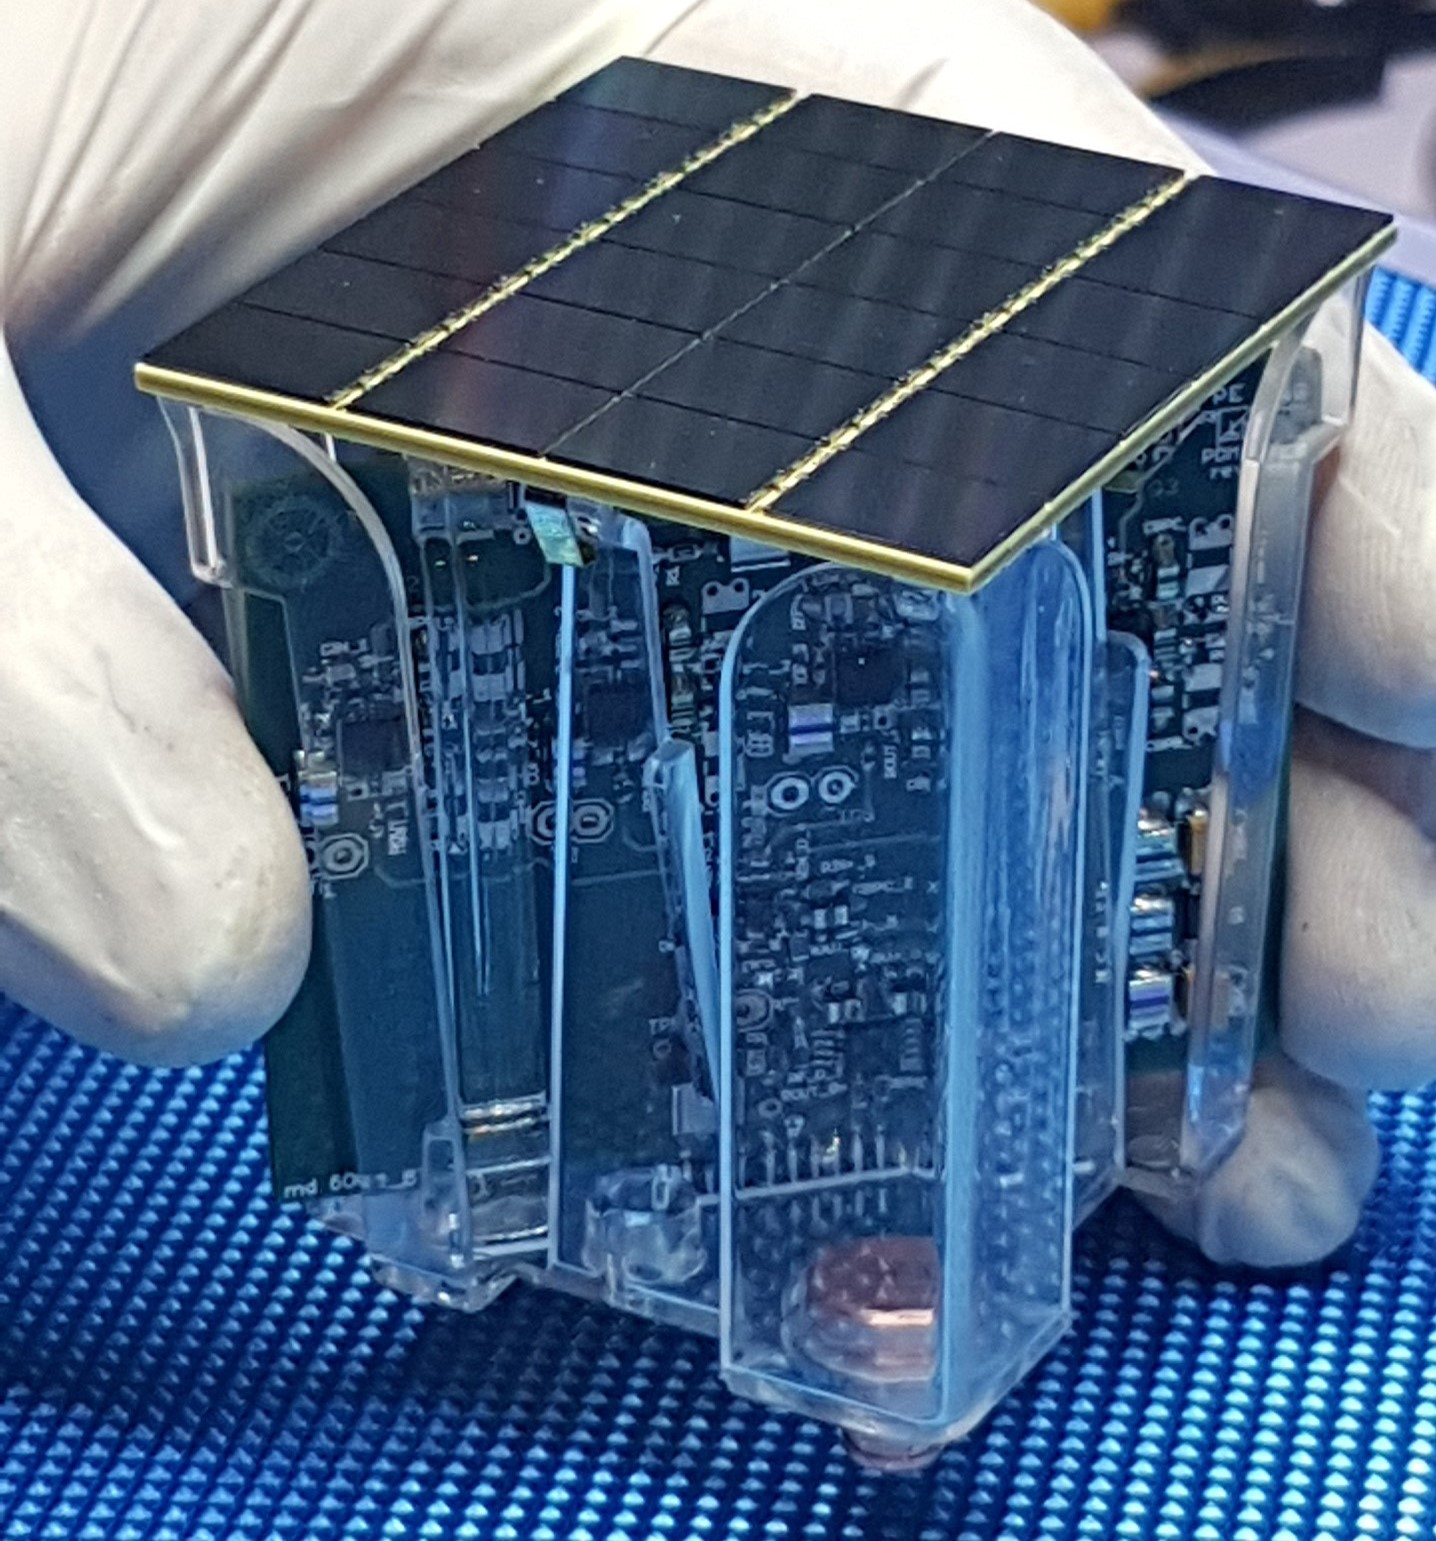
\includegraphics[width=0.49\textwidth]{./Figures/PDM-photo.jpg}
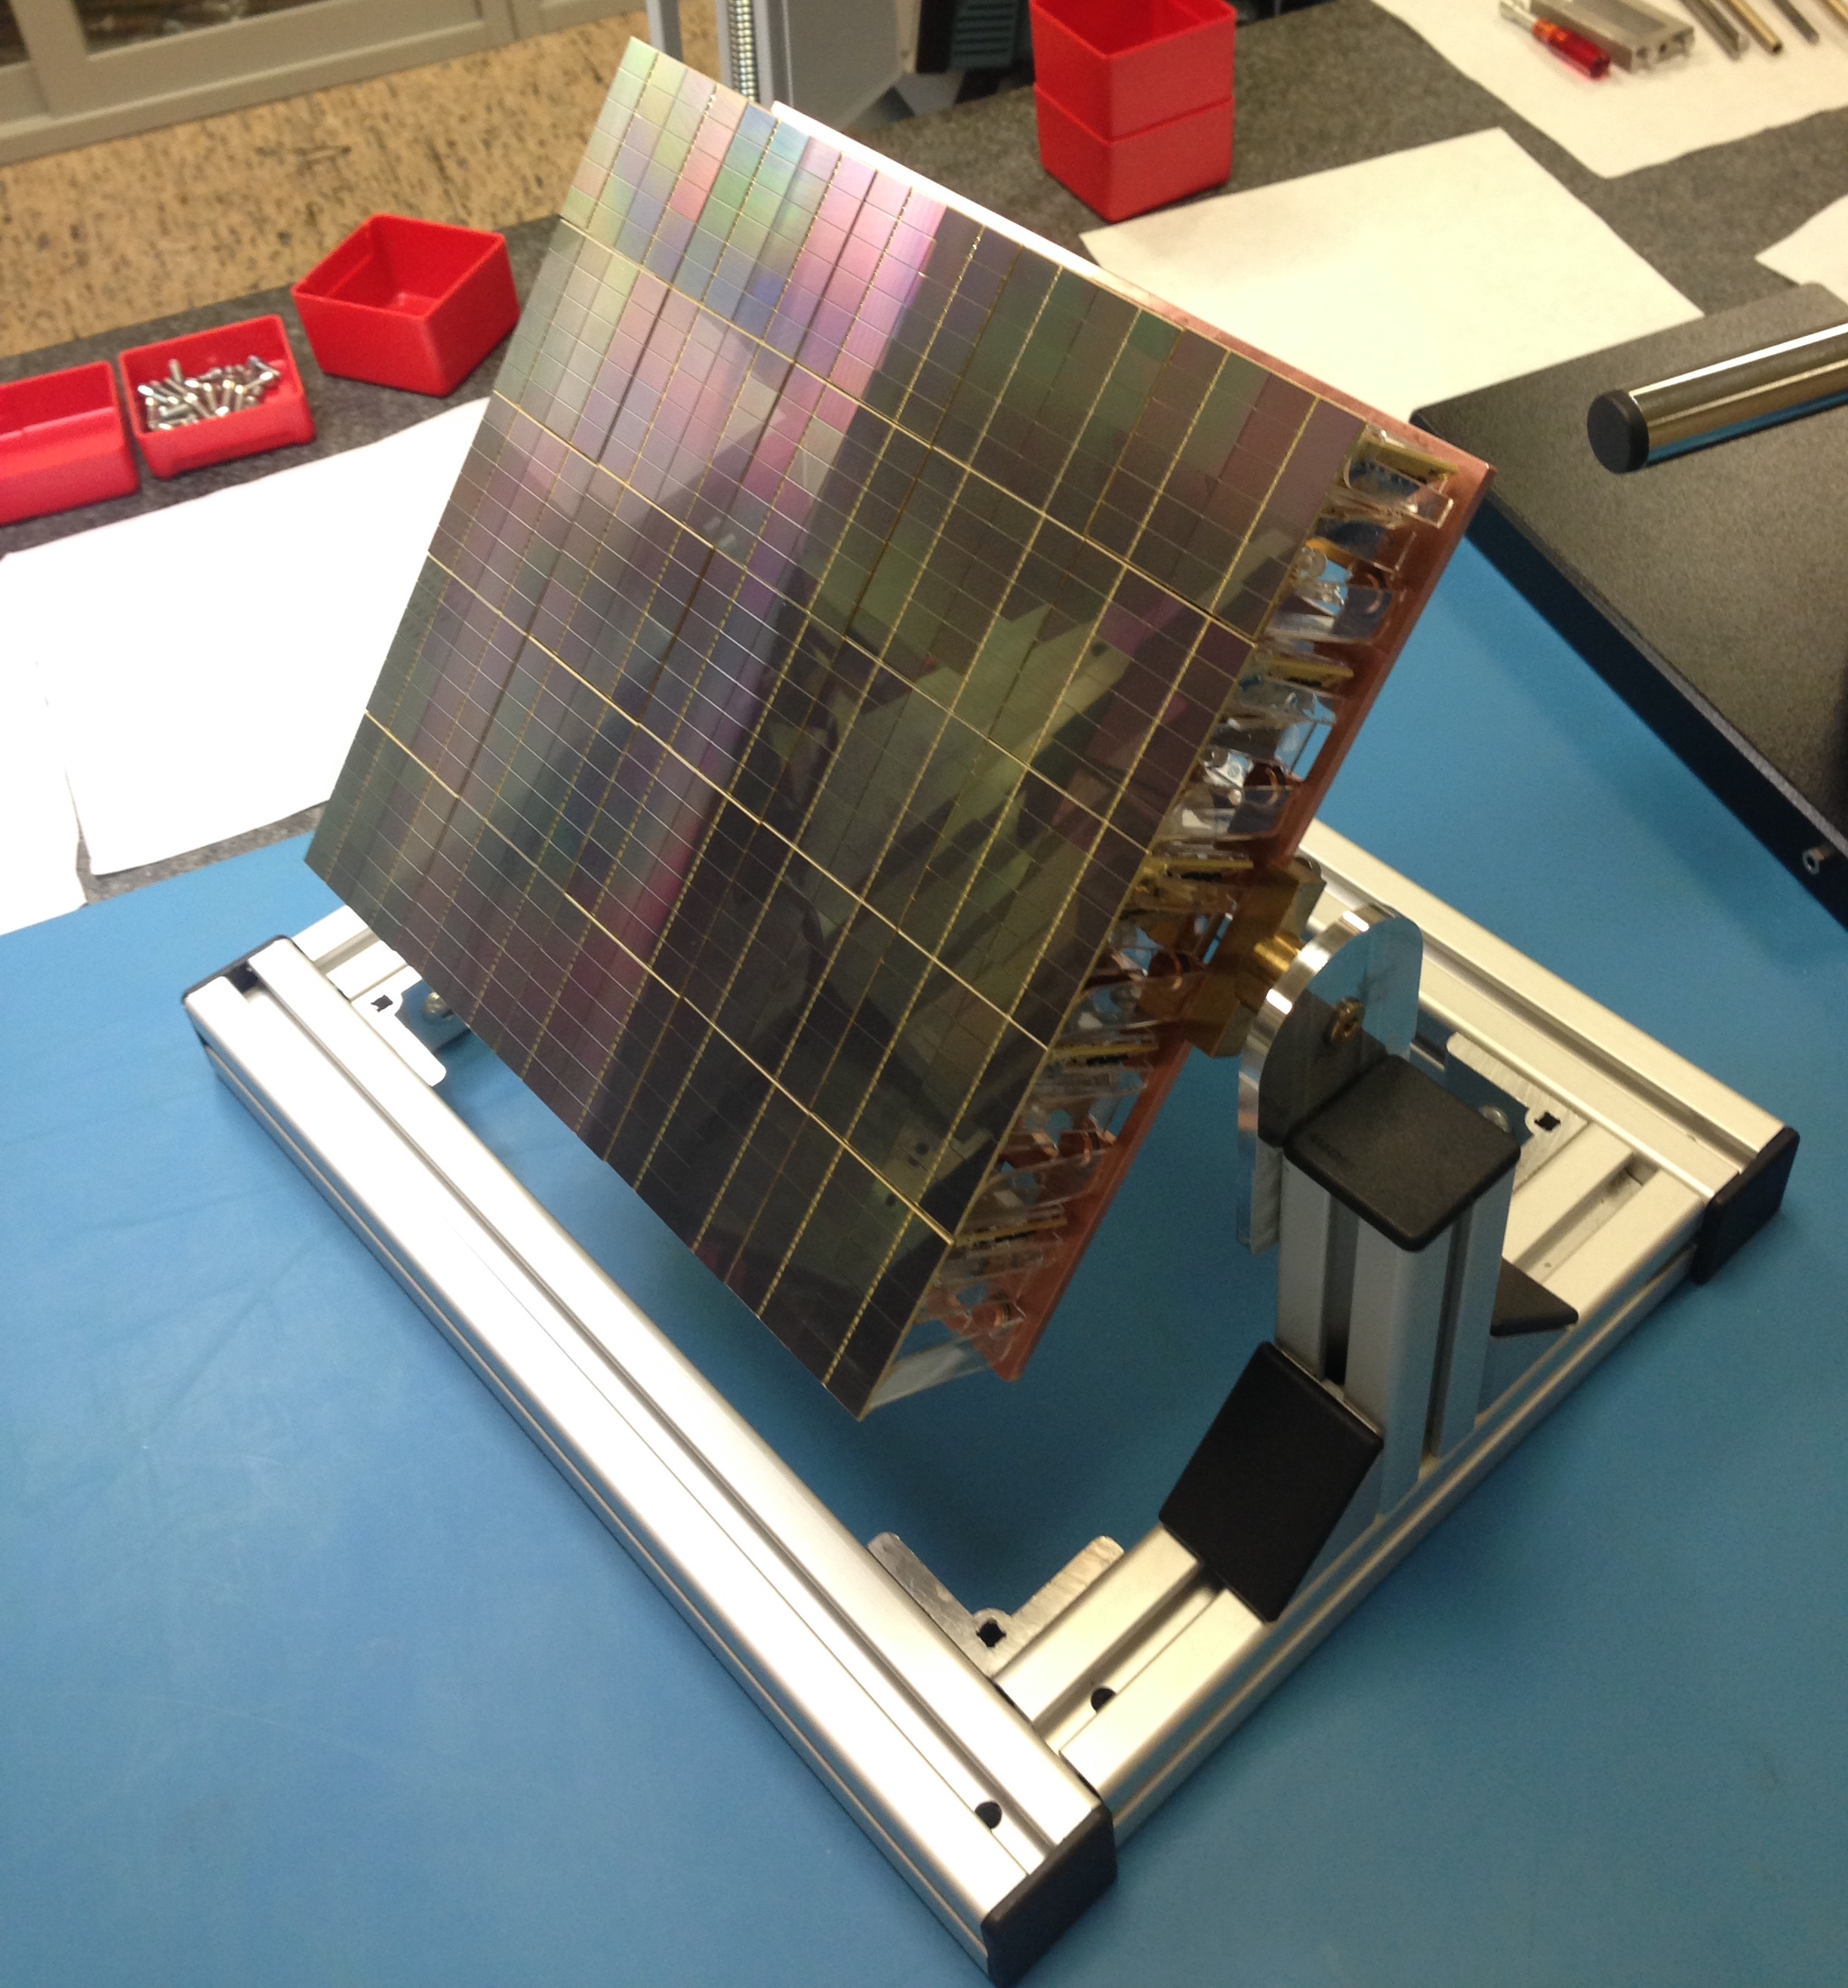
\includegraphics[width=0.49\textwidth]{./Figures/MB-photo_cut.jpg}
\caption[The first \DSkPdm\ and first motherboard resulting from the assembly of \DSkPdms]{{\bf Left:} Single channel PhotoDetector Module (\DSkPdm) consisting of   a \DSkTileAreaStd\ tile of  \DSkTileSiPMsCustomNumber\ \SiPMs\ and a front-end board.  {\bf Right:}  The \DSks\ motherboard assembled with \DSkSQBPdmsNumber\ \DSkPdms.}
\label{fig:PDM+MB}
\end{figure}


%---
\subsection{PhotoDetector Modules (\DSkPdm)}

For \DSks, the photosensing unit will be a ``PhotoDetector Module'' (\DSkPdm), consisting of a large tile of \SiPMs\ covering a total area of \DSkTileAreaStd\ operating as a single detector (see the left panel of Figure~\ref{fig:PDM+MB}).  Besides the tile, each module will also contain a cryogenic preamplifier board that will amplify and shape the signal in the immediate proximity of the sensor.  The output of the cryogenic amplifier will be passed on to a signal transmitter, also integrated into the \DSkPdm, and responsible for transmission of the signal through the cryostat penetration.  Finally, the \DSkPdm\ will also include the mechanical structure required to assemble all components and to efficiently dissipate heat in the \LAr\ target, minimizing the production of bubbles. An intelligent power distribution system is also foreseen, capable of disabling individual \DSkPdms\ in case of failure.

The unique challenge in readout presented by \SiPMs\ is mainly due to their capacitance. At \DSkSiPMCapacitancePerArea, a single \SiPM\ with a \DSkSiPMAreaStd\ surface area passes the \si{\nano\farad} scale for capacitance.  Yet, the experiment foresees a photo-sensing area of \DSkTilesArea.  The readout of a \LAr\ calorimeter faced a similar challenge, with capacitance for the individual cells often passing the \si{\nano\farad} scale~\cite{Willis:1974do}.  Early developments on \LAr\ calorimeter readout~\cite{Radeka:1974ca,Radeka:1988ku,Chase:1993dj,Chase:1997fk} demonstrated that the use of a transimpedance amplifier (\TIA) is preferable to a charge integration amplifier where the noise and rise time are very strongly affected by the large detector capacitance.  With this in mind, the \DS\ Collaboration has developed and optimized a \TIA\ (schematic is shown in the left panel of Figure~\ref{fig:TIA+2s3p}) with performance at \LArNormalTemperature\ in mind~\cite{DIncecco:2018fx}.  The specific goal was to maximize the amplification factor while preserving a stable signal bandwidth and \SNR.

The \SiPMs\ readout scheme strongly affects the PDM performance in terms both of \SNR\ and bandwidth of the signal. A hybrid readout scheme, with parallel-series combination of \SiPMs,  first introduced for the MEG experiment~\cite{Ootani:2013cn,Cattaneo:2016dq}, solves at once these two problems. In this configuration, the output signal of an individual \SiPM\ is reduced by a factor equal to the number of \SiPMs\ put in series, but this disadvantage is offset by the attenuation of the noise gain due to the reduction in the input capacitance. Most importantly, a strong improvement of the bandwidth with respect to the parallel readout scheme is achieved, with six \SiPMs\ easily readout by connecting in parallel three branches of two \SiPMs\ put in series (known as the 2s3p configuration~\cite{DIncecco:2018hy}, see right panel of Figure~\ref{fig:TIA+2s3p}) with a bandwidth comparable to the one achievable with a single \SiPM\ in input. Four such readout quadrants are fit in a single PDM, with their output signals summed at the transmission stage.

\begin{figure}[t!]
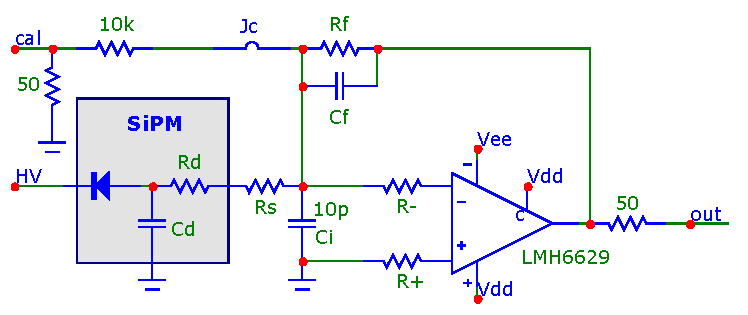
\includegraphics[width=0.49\textwidth]{./Figures/tia-schem.pdf}
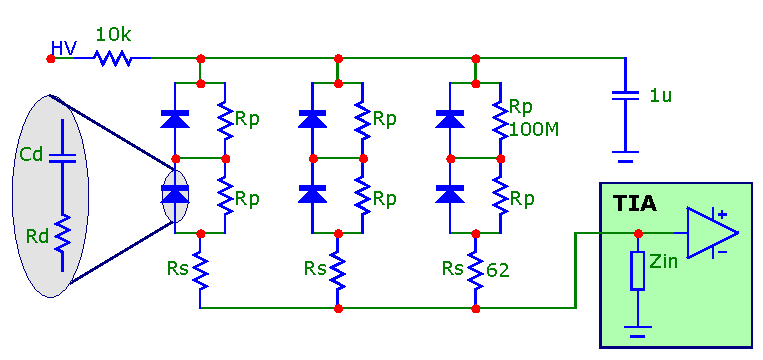
\includegraphics[width=0.49\textwidth]{./Figures/2s3p-schem.pdf}
\caption[Schematic of the transimpedance amplified and summing circuits]{{\bf Left:}  Schematic diagram of the transimpedance amplifier circuit developed to  readout \SiPMs.  {\bf Right}: Schematic diagram of the 2s3p readout scheme optimized for summing six \SiPM\ signal together.}
\label{fig:TIA+2s3p}
\end{figure}


%---
\subsection{Signal Transmission}

The signal transmission from the \DSkPdms\ to the warm electronics is of primary importance for the experiment. Given the high number of independent channels, cables would introduce a large mass in the cryostat with the inherent problems of radio-purity and heat load. The delivery of the PDM signals to the outside world through optical fibers will solve at once these two problems. For this purpose an optical analog cryogenic transmitter has been developed. The prototype boards of the opto-link system (optical driver and optical receiver board) have been recently produced. The optical receiver board (32 channels) was successfully tested, while the optical driver board (25 channels) is at the moment undergoing testing.

The \DSkPdms\ will be located above the anode and below the cathode, fully covering the top and bottom faces of the \LArTPC\ active volume, to detect both the \SOne\ and \STwo\ signals with high efficiency.  The top and the bottom photon readout assemblies will consist of \DSkTilesHalfNumber\ \DSkPdms\ each.  Multiple \DSkPdms\ are mounted to a single motherboard to form two larger basic mechanical units called the square board (\SQB)  and the triangular board (\TRB),  described in Sec.~\ref{sec:TPC} and shown  in Figure~\ref{fig:3D-TRB-SQB}.  The \SQB\ and \TRB\ have the same edge size of \DSkSQBTRBSize.  The \SQB\ and \TRB\ are then used to form the full readout planes (shown in Figure~\ref{fig:TPC-SiPM_pattern}).  The total number of readout channels (top and bottom) is \DSkTilesNumber.


%---
\subsection{\DSkPdm\ Fabrication and Characterization}

Following the successful construction of the first Photo-Detector Module (PDM) in March 2018, the Photo-Electronics Working Group proceeded to the construction of the first Motherboard, shown in  Figure~\ref{fig:PDM+MB}. The FBK company delivered two SiPM runs: the first one with standard doping SiPMs (cell size \DSkSiPMSPADSizeStd\ and quenching resistor \DSkSiPMSPADQuenchingResistorSingleDoping(\LINNormalTemperature)) and the second one with triple doping SiPMs (cell size \DSkSiPMSPADSizeTripleDoping\ and quenching resistor \DSkSiPMSPADQuenchingResistorTripleDoping(\LINNormalTemperature)). Since the latter SiPM type is considered the best candidate for the \DSks\ experiment, we decided to use the single doping SiPMs for the first Motherboard construction, so that the triple doping type could be mounted later, taking advantage of the experience gained with the mounting of the first Motherboard.

\begin{figure} [t]
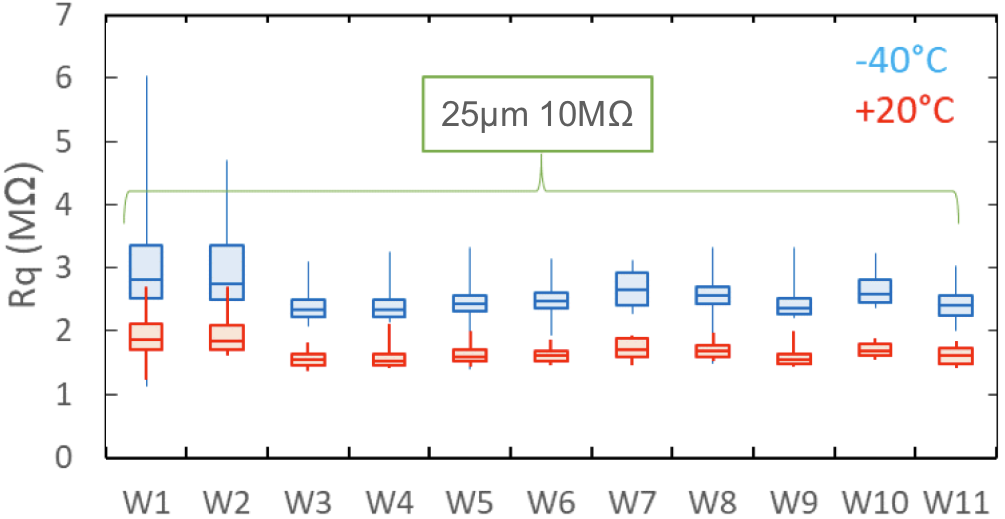
\includegraphics[width=\columnwidth]{./Figures/Rq.png}
\caption[Variance of impedance of \SiPMs\ quenching resistors]{Average \SiPM\ quenching resistor value vs. wafer number measured at \SI{20}{\celsius} and \SI{-40}{\celsius}.}
\label{fig:Rq} 
\end{figure} 

This \SiPM\ run was characterized by a reasonable yield at \SI{-40}{\celsius} of about \SI{50}{\percent}.  A detailed inspection of the SiPM quenching resistor ($R_q$) showed good uniformity for most of the wafers, while the first and the second wafers (W1,W2) had a \SI{20}{\percent} larger $R_q$ (see Figure~\ref{fig:Rq}). The optimal working voltage of the \SiPM\ is expected to change as a function of $R_q$, so in the forthcoming mass production by the LFoundry company, where hundreds of \SI{8}{\inch} SiPM wafers are scheduled, this quenching resistor spread is not an issue since the \SiPMs\ with similar $R_q$ can be paired.  In this way, each Motherboard, with \DSkPdms\ biased at the same voltage, will be made of devices with similar $R_q$. Due to the limited \SiPMs\ available in the present production we had to use all of them to make the first Motherboard, and thus all were biased with a common voltage despite the slight difference in $R_q$.  As a consequence, the tiles made with \SiPMs\ belonging to wafers~1 and~2 were fed with an overvoltage lower than the optimal one for some of the \SiPMs, i.e. \SI{5}{\volt}.  It is worth noting that a dedicated facility for the Motherboard production is not available yet, and therfore the use of equipment through outsourcing and  additional man power was therefore required.

The tile and the Front-End Board PCBs were made with an \ArlonFiveFiveNT\ substrate, following the experience gained during the first PDM construction. The electronic components were mounted with outsourced equipment, under the supervision of LNGS personnel. The tile PCBs were tested both at warm and at cryogenic temperatures to verify the correct circuit impedance. After the wafer dicing, the SiPMs were shipped from FBK to Princeton University, where the first Motherboard tiles were bonded by personnel from LNGS, Princeton University and TIFPA. A cryogenic epoxy for the SiPM back-side and a wire-bonding connection for the front-side was used. The 27 tiles, each made of \DSkTileSiPMsCustomNumber\ SiPMs, were then shipped to LNGS, using multipurpose acrylic boxes, designed by the Pisa group. This box allows for safe shipping of the tile, offering an adequate protection of the SiPM wire bonding and, at the same, time allows the tile characterization in liquid nitrogen by permitting the insertion of the Front End Board without removing the tile from the box. The tiles underwent a comprehensive test at LNGS both at warm temperature and in LN, including the reverse I-V curve measurement, the power spectrum and the charge spectra. We found just one tile out of the 27 with two SiPM branches (4 SiPMs) not working properly. Another tile showed a noise level higher than the average. These two tiles were therefore excluded from the list of the tiles selected to populate the first Motherboard.

As an example, the left side of Figure~\ref{fig:I-V-SNR} shows the tile I-V curves taken at \LINNormalTemperature, indicating a homogeneous behavior.  

\begin{figure} [t]
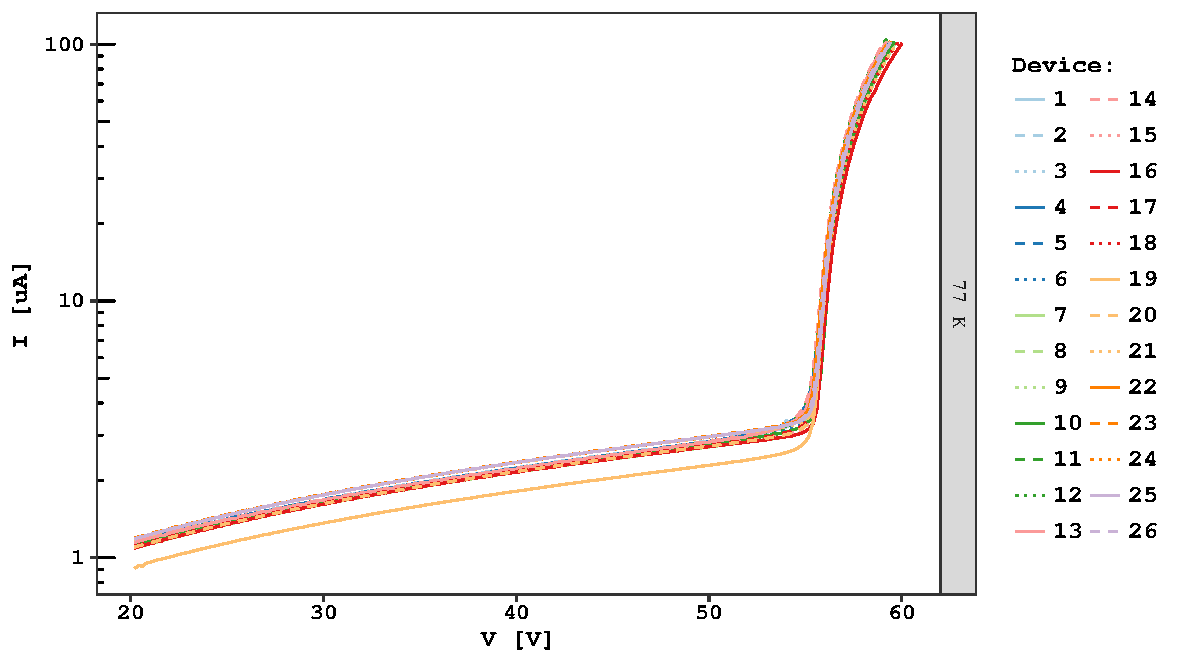
\includegraphics[width=0.49\columnwidth]{./Figures/IV_77K.pdf}
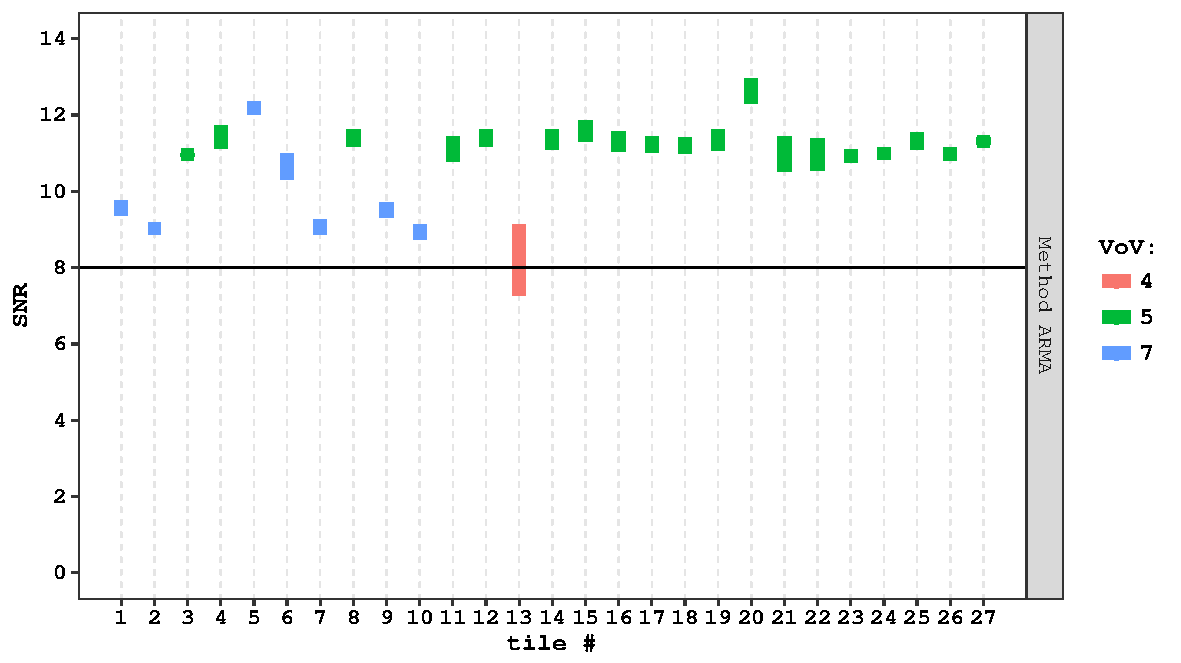
\includegraphics[width=0.49\columnwidth]{./Figures/SNR.pdf}
\caption[\SiPM\ $I$-$V$ curves and \SNR]{{\bf Left:} Reverse I-V curves for the \SiPM\ tiles measured at \LINNormalTemperature.  {\bf Right:} \SNR\ of the \num{27} bonded \SiPM\ tiles.}
\label{fig:I-V-SNR} 
\end{figure} 


The right panel of Figure~\ref{fig:I-V-SNR} shows the signal to noise ratio (\SNR) for the 27 tiles at their optimal voltage.  It is worth noting that all of them have a \SNR\ larger than the minimum \SNR\ of \DSkTileChargeSNRSpecification, required by the \DSk\ experiment specifications. For each tile, the \SNR\ was obtained relying on several different procedures and analysis methods.  The bar length in the figure represents the spread of each measurement, depending on the method used.  The signal-to-noise ratio (\SNR) is defined as the ratio between the gain and the width of the baseline noise peak. The gain is measured by fitting the center values of the amplitude multiple peaks and evaluating the slope of a linear fit. The baseline noise is extracted from the average standard deviation of the waveform in a pre-pulse window, 500 ns long, using 500 samples. For most tiles, the distribution of the standard deviation is not symmetric around the peak.  The most important contribution to the noise baseline is the presence of one or more photoelectrons not stimulated by the laser pulse. These can originate from a SiPM having an excess of dark-rate or more probably by an excess of after-pulsing.

Since the distribution is not symmetric, the estimate of the baseline noise is intrinsically biased and two options are possible, corresponding to the mean value or the most probable value (mode). Consequently the \SNR\ is defined in a confidence interval between $\SNR_{\rm min} = {\rm gain}/{\rm noise}_{\rm mean}$ and $\SNR_{\rm max} = {\rm gain}/{\rm noise}_{\rm mode}$.

Figure~\ref{fig:SNR2} shows the \SNR\ obtained with the common over-voltage of \SI{5}{\volt}. Although a few tiles, as expected, manifest a \SNR\ slightly below \DSkTileChargeSNRSpecification, the \SNR\ is quite good for all tiles used in the assembly of the first Motherboard.


%---
\subsection{Motherboard Assembly}

Before assembling the first Motherboard, a full mock-up made of an aluminum Motherboard structure, an FR4 Motherboard strip PCB, \DSkSQBPdmsNumber\ dummy tiles and FEBs, and the PDM acrylic mechanics was mounted at Bologna. Each PCB had the same dimensions of the final one, while the HV/LV and signal layers were not included in the stack-up. The mounting required just a few hours and the overall procedure was validated, while the mechanics of the different components nicely merged, suggesting just a few minor mechanical improvements. 

After these tests, the tiles were finally shipped to Pisa, while the \DSkPdm\ pillars and the copper Motherboard structure were milled at Bologna using \SI{99.997}{\percent} pure copper sold by the Luvata Company. The first Motherboard was equipped with a PCB strip connecting the \DSkPdms, made of a thin stack-up (\SI{0.5}{\milli\meter}) based on a Pyralux substrate and shipped to Pisa to start the mounting of the \DSkSQBPdmsNumber\ \DSkPdms\ on the Motherboard. 

The \DSkPdms\ were assembled in the Pisa clean room, following the prescriptions used for the first \DSkPdm, assembled in March 2018. The mounting of the \DSkSQBPdmsNumber\ \DSkPdms\ on the Motherboard was finalized in few days.  A picture of the first Motherboard, fully equipped with the first \DSkSQBPdmsNumber\  \DSkPdms\ is shown in the right panel of Figure~\ref{fig:PDM+MB}.

In summary the construction of the first Motherboard required the production, testing, selection and bonding of more than 600 \SiPMs. Although a cryogenic probe and an automatic bonder were not available yet, the Collaboration was able to increase the number of successfully built \DSkPdms\ from 1 to \DSkSQBPdmsNumber, in just \num{6} months. The bonding yield exceeded \SI{95}{\percent} (just 1 tile out of the 27 showed problems with the \SiPM\ bonding strategy), while the satisfactory \DSkPdm\ \SNR\ demonstrated the validity of the full Motherboard construction process.

After the completion of the first motherboard, equipped with \DSkSQBPdmsNumber\ \DSkPdms\ each containing  \DSkTileSiPMsCustomNumber\ single dose SiPM's, the collaboration moved to the construction of a second Motherboard, equipped with triple dose \SiPMs.   At the moment, half of the \DSkPdms\ have already been assembled and mounted in the copper structure. The remaining \DSkPdms\ will be mounted within the summer of~2019.  The FEBs were already successfully tested, while the \SiPM\ tiles are currently undergoing testing in LN. The next step in the photo-electronics schedule is the production of about  \DSkPdmsSecondBatchNumber\ \DSkPdms\ for the \DSps\ detector. These \SiPMs\ will be produced by the LFoundry Company in Avezzano, Italy.  The first run is expected in the summer of~2019. 

\begin{figure}[t!]
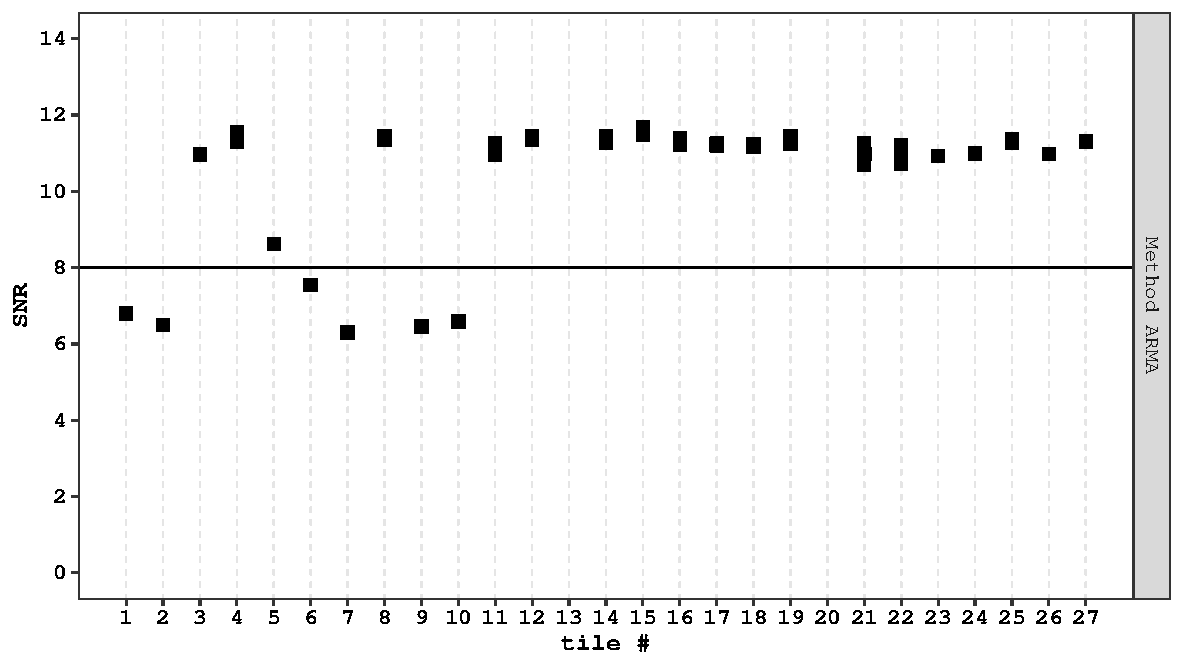
\includegraphics[width=0.5\columnwidth]{./Figures/SNR2.pdf}
\caption[\SNR\ of the \SiPMs\ tiles of the first motherboard]{\SNR\ of the \DSkSQBPdmsNumber\ \SiPM\ tiles populating the first motherboard while.  Data were recorded while operating the \SiPM\ tiles at an over-voltage of \SI{5}{\volt}.}
\label{fig:SNR2} 
\end{figure} 


%---
\subsection{Mass Production}

The first engineering run, finalized in September 2018 and tested shortly after, showed the capability of the silicon foundry to implement the FBK technology.  The produced \SiPMs\ showed good performance at both room temperature and in liquid nitrogen. A second LFoundry engineering run, presently ongoing, is devoted to the development of the through silicon vias (TSV). This post-production rework requires some delicate mechanical manipulation of the SiPM wafers.

The \DSks\ \SiPM\ packaging foresees the production of more than \DSkPdmsNumberWithSpares\ \DSkPdms\ in \DSkPdmsContructionTime. This remarkable effort requires a large clean room, relying on cutting edge technology equipment and trained personnel.  The \GADMC\ selected for the \NOA\ \DSks\ \SiPM\ packaging facility a clean room at the {\it Tecnopolo dell'Aquila}, with surface exceeding \DSkPdmsCleanRoomSurface.  The clean room will be soon refurbished to comfortably host the needed equipment and personnel.  This facility will be managed by \GSSI, through an agreement with \INFN\ that will soon be finalized.  Concerning the procurement of the equipment for the \DSks\ \DSkPdms\ mass production, the cryogenic probe tender was just approved by the \INFN\ Executive Board and the flip-chip bonder tender will follow in the weeks to come.